% !TEX root = ../AiiDA_tutorial.tex
\section[Verdi command line]{Using the verdi command line}

This part of the tutorial will help to familiarize you with the command-line utility \cmd{verdi}, one of the most common ways to interact with AiiDA. \cmd{verdi} with its subcommands enables a variety of operations such as inspecting the status of ongoing or terminated calculations, showing the details of calculations, computers, codes, or data structures, access the input and the output of a calculation, etc.  Similar to the \texttt{bash} shell, verdi command support Tab completion. Try right now to type \cmd{verdi} in a terminal and tap Tab twice to have a list of subcommands. Whenever you need the explanation of a command type \cmd{verdi help} or add \cmd{-h} flag if you are using any of the \cmd{verdi} subcommands. 
Finally, fields enclosed in angular brackets, such as \texttt{<pk>}, are placeholders to be replaced by the actual value of that field (an integer, a string, etc...).

\subsection{The list of calculations}
Let us try our first \cmd{verdi} commands. Type in the terminal
\begin{bashcommand}
verdi calculation list
\end{bashcommand}
(Note: the first time you run this command, it might take a few seconds as it is the first time you are accessing the database in the virtual machine. Subsequent calls will be faster).
This will print the list of ongoing calculations, which should be empty. The first output line should look like
\begin{verbatim}
PK    Creation    State    Type    Computer    Job state
----  ----------  -------  ------  ----------  -----------

Total results: 0

Info: last time an entry changed state: never
\end{verbatim}

In order to print a list with all calculations that finished correctly in the AiiDA database, you can use the \cmd{-s/-{}-states} flag as follows:
\begin{bashcommand}
verdi calculation list --states FINISHED
\end{bashcommand}
Another very typical option combination allows to get calculations in \emph{any} state (flag \cmd{-a}) generated in the past \cmd{NUM} days (\cmd{-p <NUM>}): e.g., for calculation in the past 1 day: \cmd{verdi calculation list -p1 -a}. Since you have not yet run any calculations at the virtual machine that you currently use and all the existing calculations were imported and belong to a different user, you can type (flag \cmd{-A} shows the calculations of all the users):
\begin{bashcommand}
verdi calculation list -A --states IMPORTED
\end{bashcommand}

Each row of the output identifies a calculation and shows some information about it. For a more detailed list of properties, choose one row by noting down its PK (primary key) number (first column of the output) and type in the terminal 
\begin{bashcommand}
verdi calculation show <pk>
\end{bashcommand}
The output depends on the specific pk chosen and should inform you about the input nodes (e.g. pseudopotentials, kpoints, initial structure, etc.), and output nodes (e.g. output structure, output parameters, etc.). 

\begin{tcolorbox}
\textbf{PKs/IDs vs.\@ UUIDs}: Beside the (integer) PK, very convenient to reference a calculation or data node
in your database, every node has a UUID (Universally Unique ID) to identify it, that is preserved even when you share some nodes with coworkers---while the PK
will most likely change. You can see the UUID in the output of \texttt{verdi calculation show} or \texttt{verdi node show}. Moreover, if you have already a UUID and you want
to get the corresponding PK in your database, you can use \texttt{verdi node show -u <UUID>},
as we are going to do now.
\end{tcolorbox}

Let us now consider the node with \texttt{UUID = ce81c420-7751-48f6-af8e-eb7c6a30cec3}, which identifies a relaxation of a BaTiO$_3$ unit cell run with Quantum Espresso \cmd{pw.x}.
You can check the information on this node and get the PK with:
\begin{verbatim}
$ verdi node show -u ce81c420-7751-48f6-af8e-eb7c6a30cec3
Property       Value
-------------  ------------------------------------
type           PwCalculation
pk             4235
uuid           ce81c420-7751-48f6-af8e-eb7c6a30cec3
label
description
ctime          2014-10-27 17:51:21.781045+00:00
mtime          2018-05-16 11:19:39.848446+00:00
process state
finish status
computer       [2] daint
code           pw-SVN-piz-daint

Inputs        PK  Type
----------  ----  -------------
parameters  4236  ParameterData
kpoints     4526  KpointsData
pseudo_Ba    966  UpfData
pseudo_Ti   4315  UpfData
settings    4529  ParameterData
pseudo_O    4342  UpfData
structure    436  StructureData

Outputs                    PK  Type
-----------------------  ----  -------------
output_kpoints           3665  KpointsData
output_parameters        3670  ParameterData
output_structure         3666  StructureData
retrieved                3668  FolderData
output_trajectory_array   265  ArrayData
remote_folder            1977  RemoteData
\end{verbatim}
\emph{Keep in mind that you can also use just a part (beginning) of the UUID, as long as it is unique, to show the node information information.} For example, to display the above information, you could also type \cmd{verdi node show -u ce81c420}. In what follows, we are going to mention only the prefixes of the UUIDs since they are sufficient to identify the correct node.

\subsection{A typical AiiDA graph}
\label{sec:aiida_graph}
AiiDA stores inputs required by a calculation as well as the its outputs in the database. These objects are connected in a graph that looks like Fig.~\ref{fig:graph}. We suggest that you have a look to the figure before going ahead.

\begin{figure}
\centering
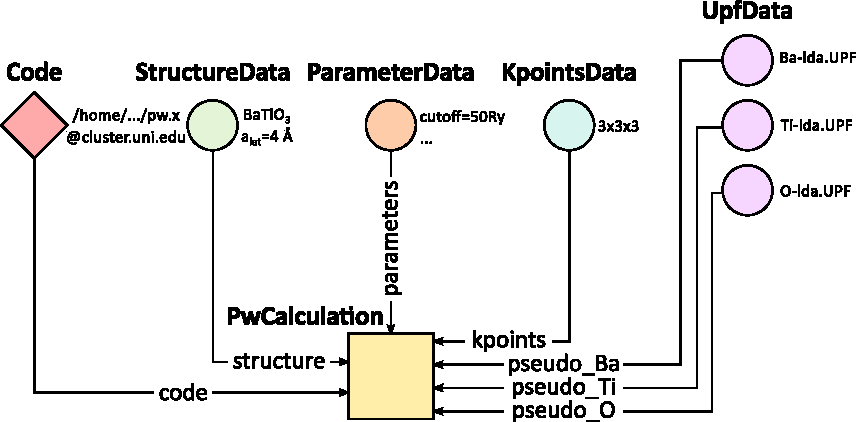
\includegraphics[width=0.5\textwidth]{img/graph/graph-inputonly}

\vspace {1cm}
 
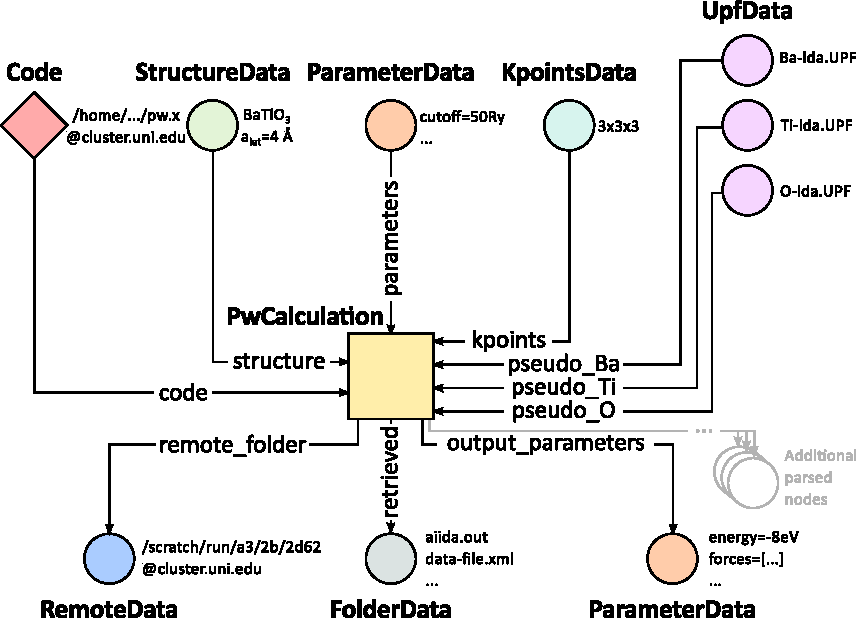
\includegraphics[width=0.5\textwidth]{img/graph/graph-full}
\caption{\label{fig:graph}\textbf{(a, top)} Graph with all inputs (data, circles; and code, diamond) to the Quantum Espresso calculation (square) that you will create in Sec.~\ref{sec:qe} of this tutorial. \textbf{(b, bottom)} Same as (a), but also with the outputs that the daemon will create and connect automatically. The RemoteData node is created during submission and can be thought as a symbolic link to the remote folder in which the calculation runs on the cluster. The other nodes are created when the calculation has finished, after retrieval and parsing. The node with linkname ``retrieved'' contains the raw output files stored in the AiiDA repository; all other nodes are added by the parser. Additional nodes (symbolized in gray) can be added by the parser (e.g., an output StructureData if you performed a relaxation calculation, a TrajectoryData for molecular dynamics, \ldots).}
\end{figure}

You can create a similar graph for any calculation node by using the utility \cmd{verdi graph generate <pk>}. For example, before you obtained information (in text form) for \texttt{UUID = ce81c420}. To visualize similar information in graph(ical) form, run (replacing \cmd{<pk>} with the PK of the node):
\begin{bashcommand}
verdi graph generate <pk>
\end{bashcommand}

This command will create the file \texttt{<pk>.dot} that can be rendered by means of the utility \cmd{dot}. If you now type 
\begin{bashcommand}
dot -Tpdf -o <pk>.pdf <pk>.dot
\end{bashcommand}
you will create a pdf file \texttt{<pk>.pdf}. You can open this file on the Amazon machine by using \cmd{evince} or, if you feel that the ssh connection is too slow, copy it via \cmd{scp} to your local machine.
To do so, if you are using Linux/Mac OS X, you can type in your \emph{local} machine:
\begin{bashcommand}
scp aiidatutorial:<path_with_the_graph_pdf> <local_folder>
\end{bashcommand}
and then open the file. Alternatively, you can use graphical software to achieve the same, for instance: WinSCP on Windows, Cyberduck on the Mac, or the ``Connect to server'' option in the main menu after clicking on the desktop for Ubuntu.

Spend some time to familiarize yourself with the graph structure. Choose the root node (highlighted in blue) and trace back the parent calculation which produced the structure used as an input. This is an example of a Quantum ESPRESSO pw.x calculation, where the input structure was actually obtained as the output of a previous calculation. We will now inspect the different elements of this graph.

\subsection{Inspecting the nodes of a graph}
\subsubsection*{ParameterData and Calculations}
Now, let us have a closer look at the some of the nodes appearing in the graph. 
Choose the node of the type \texttt{ParameterData} with input link name \texttt{parameters}
(to double check, it should have UUID \texttt{d1bbe1ea}) 
and type in the terminal:
\begin{bashcommand}
verdi data parameter show <pk>
\end{bashcommand}
A \texttt{ParameterData} contains a dictionary (i.e., key--value pairs), stored in the database in a format ready to be queried (we will learn how to run queries later on in this tutorial). The command above will print the content dictionary, containing the parameters used to define the input file for the calculation. You can compare the dictionary with the content of the raw input file to Quantum ESPRESSO (that was generated by AiiDA) via the command
\begin{bashcommand}
verdi calculation inputcat <pk>
\end{bashcommand}
where you substitute the pk of the calculation node. 
Check the consistency of the parameters written in the input file and those stored in the ParameterData node. Even if you don't know the meaning of the input flags of a Quantum ESPRESSO calculation, you should be able to see how the input dictionary
has been converted to Fortran namelists. 

The previous command just printed the content of the ``default'' input file \texttt{aiida.in}. 
To see a list of all the files used to run a calculation (input file, submission script, etc.) instead type
\begin{bashcommand}
verdi calculation inputls <pk>
\end{bashcommand}
(Adding a \texttt{-{}-color} flag allows you to easily distinguish files from folders by a different coloring).

Once you know the name of the file you want to visualize, you can call the \cmd{verdi 
calculation inputcat} command specifying the path. For instance, to see the submission
script, you can do:
\begin{bashcommand}
verdi calculation inputcat <pk> -p _aiidasubmit.sh
\end{bashcommand}

%%%%%%%%%%%%%%%%%%%%%%Structure data%%%%%%%%%%%%%%%%%%%
\subsubsection*{StructureData}
Now let us focus on StructureData objects, representing a crystal structure.
We can consider for instance the input structure to the calculation we were 
considering before (it should have UUID prefix \texttt{3a4b1270}).
Such objects can be inspected interactively by means of an atomic viewer such as the one provided by \texttt{ase}. AiiDA however supports several other viewers such as \texttt{xcrysden}, \texttt{jmol}, and \texttt{vmd}. Type in the terminal 
\begin{bashcommand}
verdi data structure show --format ase <pk>
\end{bashcommand}
to show the selected structure (it will take a few seconds to appear, and you can rotate the view with the right mouse button---if
you receive some errors, make sure you started your SSH connection with the 
\texttt{-X} or \texttt{-Y} flag).

Alternatively, especially if showing them interactively is too slow over SSH, you can export the content of a structure node in various popular formats such as \texttt{xyz} or \texttt{xsf}. This is achieved by typing in the terminal
\begin{bashcommand}
verdi data structure export --format xsf <pk>  >  <pk>.xsf
\end{bashcommand}
You can open the generated \texttt{xsf} file and observe the cell and the coordinates. Then, you can then copy \texttt{<pk>.xsf} from the Amazon machine to your local one and then visualize it, e.g. with xcrysden (if you have it installed):
\begin{bashcommand}
xcrysden --xsf <pk>.xsf
\end{bashcommand}

%%%%%%%%Verdi code%%%%%%%%%%%%
\subsubsection*{Codes and computers}
Let us focus now on the nodes of type \texttt{code}. A code represents (in the database) the actual executable used to run the calculation. Find the pk of such a node in the graph and type
\begin{bashcommand}
verdi code show <pk>
\end{bashcommand}

The command prints information on the plugin used to interface the code to AiiDA, the remote machine on which the code is executed, the path of its executable, etc. To show a list of all available codes type
\begin{bashcommand}
verdi code list
\end{bashcommand}
If you want to show all codes, including hidden ones and those created by other users, use \texttt{verdi code list -a -A}. Now, among the entries of the output you should also find the code just shown.

%%%%%%%%%%%Verdi computer%%%%%%%%%%
Similarly, the list of computers on which AiiDA can submit calculations is accessible by means of the command
\begin{bashcommand}
verdi computer list -a
\end{bashcommand}
(\cmd{-a} shows all computers, also the one imported in your database but that you did not configure, i.e., to which you don't have access).
Details about each computer can be obtained by the command 
\begin{bashcommand}
verdi computer show <COMPUTERNAME>
\end{bashcommand}
Now you have the tools to answer the question:
\begin{tcolorbox}
What is the scheduler installed on the computer where the calculations of the graph have run?
\end{tcolorbox}


%%%%%%%%%%%%%%%verdi output|res%%%%%%%%%%%%%%%%
\subsubsection*{Calculation results}
The results of a calculation can be accessed directly from the calculation node. Type in the terminal
\begin{bashcommand}
verdi calculation res <pk>
\end{bashcommand}
which will print the output dictionary of the ``scalar'' results parsed by AiiDA at the end of the calculation.  Note that this is actually a shortcut for 
\begin{bashcommand}
verdi data parameter show <pk2>
\end{bashcommand}
where \texttt{pk2} refers to the ParameterData node attached as an output of the calculation node, with link name \texttt{output\_parameters}.

\begin{tcolorbox}
By looking at the output of the command, what is the Fermi energy of the calculation with UUID prefix \texttt{ce81c420}?
\end{tcolorbox}



%%%%%%%%%%%%verdi output cat%%%%%%%%%%%
Similarly to what you did for the calculation inputs, you can access the output files via the commands
\begin{bashcommand}
verdi calculation outputls <pk>
\end{bashcommand}
and
\begin{bashcommand}
verdi calculation outputcat <pk>
\end{bashcommand}
Use the latter to verify that the Fermi energy that you have found in the last step has been extracted correctly from the output file (Hint: filter the lines containing the string ``Fermi'', e.g. using \texttt{grep}, to isolate the relevant lines). 

%%%%%%%%%%%verdi data array show%%%%%%%%%%%%
The results of calculations are stored in two ways: \texttt{ParameterData} objects are stored in the database, which makes querying them very convenient, whereas \texttt{ArrayData} objects are stored on the disk. Once more, use the command \cmd{verdi data array show <pk>} to know the Fermi energy obtained from calculation with UUID prefix \texttt{ce81c420} (you need to use, this time, the PK of the output ArrayData of the calculation, with link name \cmd{output\_trajectory\_array}). As you might have realized the difference now is that the whole series of values of the Fermi energy calculated after each relax/vc-relax step are stored. (The choice of what to store in \texttt{ParameterData} and \texttt{ArrayData} nodes is made by the parser of \texttt{pw.x} implemented in the \texttt{aiida-quantumespresso} plugin.)

%%%%%%%%%%%verdi comments%%%%%%%%%%%%%%5
\subsubsection*{(Optional section) Comments}
AiiDA offers the possibility to attach comments to a calculation node, in order to be able to remember more easily its details. Node with UUID prefix ce81c420 has no comment already defined, but you can add a very instructive one by typing in the terminal
%%%%%%%%%%verdi comment%%%%%%%%%%%%%%
\begin{bashcommand}
verdi comment add -c "vc-relax of a BaTiO3 done with QE pw.x" <pk>
\end{bashcommand}
Now, if you ask for a list of all comments associated to that calculation by typing
\begin{bashcommand}
verdi comment show <pk>
\end{bashcommand}
the comment that you just added will appear together with some useful information such as its creator and creation date. We let you play with the other options of \cmd{verdi comment} command to learn how to update or remove comments.


% %%%%%%%%%%TO BE DISCUSSED%%%%%%%%%%%%%%%%%%
% \textcolor{red}{We might discuss the \cmd{verdi node repo ls|cat command} e.g.}
% \begin{bashcommand}
% verdi node repo cat -p 4079 raw_input/aiida.in 
% \end{bashcommand}
% \textcolor{red}{Moreover, at this state no RemoteData concept has been introduced}


\subsection{AiiDA groups of calculations}
In AiiDA, calculations (and more generally nodes) can be organized in groups, which are particularly useful to assign a set of calculations or data to a common project. This allows you to have quick access to a whole set of calculations with no need for tedious browsing of the database or writing complex scripts for retrieving the desired nodes. Type in the terminal
\begin{bashcommand}
verdi group list
\end{bashcommand}
to show a list of the groups that already exist in the database. Choose the PK of the group named \texttt{tutorial\_pbesol} and look at the calculations that it contains by typing
\begin{bashcommand}
verdi group show <pk>
\end{bashcommand}
In this case, we have used the name of the group to organize calculations according to the pseudopotential that has been used to perform them. Among the rows printed by the last command you will be able to find the calculation we have been inspecting until now. 

If, instead, you want to know all the groups to which a specific node belomngs, you can run 
\begin{bashcommand}
verdi group list --node <pk> 
\end{bashcommand}

